\documentclass{article}
\usepackage{amsmath,mathtools,amstext,array,cases,biblatex,float,tikz}
\addbibresource{biblio-ch2.bib}

\usetikzlibrary{calc,matrix,decorations.markings,decorations.pathreplacing}
\usetikzlibrary{positioning}

\definecolor{colone}{gray}{0.7}
\definecolor{coltwo}{gray}{0.6}
\definecolor{colthree}{gray}{0.5}
\definecolor{colfour}{gray}{0.9}
\definecolor{colfive}{gray}{0.9}
\definecolor{colsix}{gray}{0.9}
\definecolor{colseven}{gray}{0.9}

\tikzset{ 
table/.style={
  matrix of nodes,
  row sep=-\pgflinewidth,
  column sep=-\pgflinewidth,
  nodes={rectangle,text width=2cm,align=center},
  text depth=1.25ex,
  text height=2.5ex,
  nodes in empty cells}
}

\tikzstyle{startstop} = [rectangle, minimum width=2cm, minimum height=1.5cm,text centered, draw=black]
\tikzstyle{process} = [rectangle, minimum width=3cm, minimum height=1.5cm, text centered, draw=black]
\tikzstyle{arrow} = [thick,->,>=stealth]

\begin{document}


\title{Chapter 2}

\author{M. Repetto}

\date{\today}

\maketitle

\begin{abstract}
In the following paper is proposed a multi-objective model for components allocation in a Green Supply Chain framework. The model builds on the concept of the supply chain as suggested by Porter, and accounts for the costs of production using the Activity Based Cost accounting method (ABC). Such model is organized in blocks related to several moments in the value chain in a sequential fashion. Above each and every one of these blocks, we included a series of environmental constraints that the firm has to comply, with respect to specific country regulation or in case of a particular corporate policy...
\end{abstract}

\section{Introduction}
Global Supply Chain Management (GSCM) is probably one of the most used terms when we talk about how the firms are running their business nowadays. GSCM may be defined as the allocation of goods and services along a series of transnational companies' global network to maximize profits and minimize waste. Inside this very wide concept, we can find the concept of logistics which is in charge of the movement of goods, service and last but not least information from the sourcing of raw material, till it reaches the end customer.
Along with these two concepts a third one stuck with them, the concept of Green Supply Chain (GSC). This concept brought to light by a more advanced concern about environmental matters of the developed countries forced the firms to be accountable for their negative externalities related to the environment in which they operate \cite{srivastava_green_2007}. 

However such legislations lack from a point of view of legal constraints, setting only a few qualitative restriction, poorly measurable toward enterprises or in some cases letting the customers pay for their environmental behavior toward waste disposition. These facts are inevitably leaving some degrees of freedom to the firms, on the other hand, is also important to notice that these are only seeds of legislation that shows us how the long-term trend will be about the tolerance given to the behavior of firms toward environmental concerns, a trend that in the future may require firms to set particular frameworks to be accountable for their environmental impact.

Because of that we propose a Goal Programming model in order to address such problem, following what proposed by literature we try to enhance such model fixing quantitative constraints to the pollution generated by the production activity involved in the creation of a good and we also try to implement the benefits of a recycling program enacted by the firm apropos the WEEE directive.

In our case, we chose the networking electronic appliance business (i.e. hub, switch or router). In order to measure such impact, we'll use the framework used by Activity Based Costing in order to assess the marginal environmental impact of any additional unit elaborated by the transnational firms in order to ultimately market the product on its reference market.

\section{Green Supply Chain}
Green Supply Chain may be defined as the series of interconnected activities across the border of different enterprises that adds value to the goods and services from the sourcing to the market. Whereas Supply Chain Management sets its objective to maximize profits and minimizes waste Green Supply Chain sets its objectives even further, posing has its ultimate mission to lower the ecological impact that a firm or a series of them has in their day to day operations. Such operation may involve:
\begin{itemize}
    \item Green manufacturing and remanufacturing: is the process of controlling and reutilizing of material in the manufacturing in order to limit waste creation\cite{urvashi_green_2013};
    \item Green design: is an approach put in place to promote the environmental quality of a certain product or service  by reducing negative impacts on the natural environment, an example could be the automatic switch off of the television after a period of idleness\cite{ceschin_evolution_2016}; and
    \item Green operations in general: by green operation, we mean any type of activity which does not fall into the two categories mentioned above but is characterized by a "green" attitude as for example the optimization of the offices' consumptions thorough a remote-working policy;
\end{itemize}

 It's worth noting that even though CEO and firms manager are looking for greener supply chain this doesn't mean that such interest was created by an increase in corporate social responsibility but more because of the legislation (in particular the European one) that seemed to be interested in guarantees a certain level of environmental quality to its citizens.

In the market under scope which is the European one, there are several legislations concerning the environmental impact of certain e-products. The most important are:
\begin{itemize}
    \item Waste Electrical \& Electronic Equipment (WEEE);
    \item Restriction on Hazardous Substances (RoHS);and
    \item Ecodesign Requirement for Energy-using Product (EuP);
\end{itemize}

Such legislation acts at different levels from the sourcing to the costumer involving community member States. The following flow chart illustrates this differences:

\begin{figure}
\centering

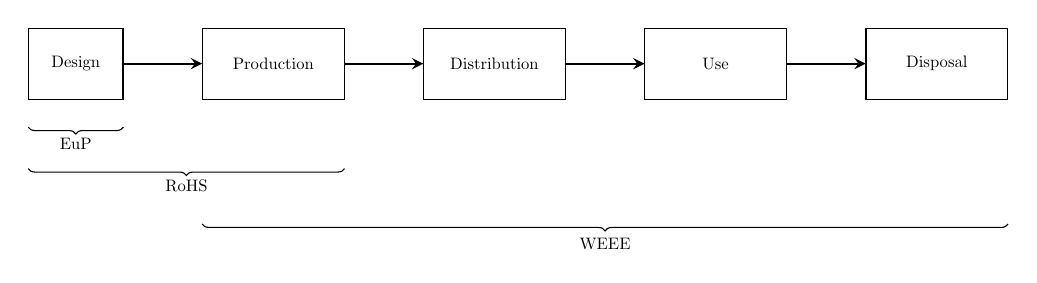
\begin{tikzpicture}[scale=0.8, every node/.style={scale=0.6}]
\node (start) [startstop] {Design};
\node (process1) [process, right=of start] {Production};
\node (process2) [process, right=of process1] {Distribution};
\node (process3) [process, right=of process2] {Use};
\node (process4) [process, right=of process3] {Disposal};

\draw [arrow] (start)--(process1);
\draw [arrow] (process1)--(process2);
\draw [arrow] (process2)--(process3);
\draw [arrow] (process3)--(process4);

\draw[decorate,decoration={brace,mirror,raise=10pt}]
  (start.south west) -- (start.south east) node[below, midway, yshift = -20]  {EuP};
\draw[decorate,decoration={brace,mirror,raise=25pt}]
  (start.south west) -- (process1.south east) node[below, midway, yshift = -45]  {RoHS};
\draw[decorate,decoration={brace,mirror,raise=45pt}]
  (process1.south west) -- (process4.south east) node[below, midway, yshift = -80]  {WEEE};

\end{tikzpicture}
\caption{Legislation affection}
\end{figure}



In the following sub section an additional overview is given to such legislations.

\subsection{Waste Electrical \& Electronic Equipment}
The Waste Electrical \& Electronic Equipment also calle WEEE is ruled in the European Community by Directive 2002/96/EC now repealed by the Directive 2012/19/EU. The objectives of the policy are, to preserve, protect and improve the quality of the environment, to protect human health and to utilise natural resources prudently and rationally. That policy is based on the precautionary principle meaning that the polluter should pay for its damage.

\subsection{Restriction on Hazardous Substances}
\subsection{Ecodesign Requirement for Energy-using Product}

\section{A state of the art review}

\section{Model formulation}


\begin{figure}
\centering

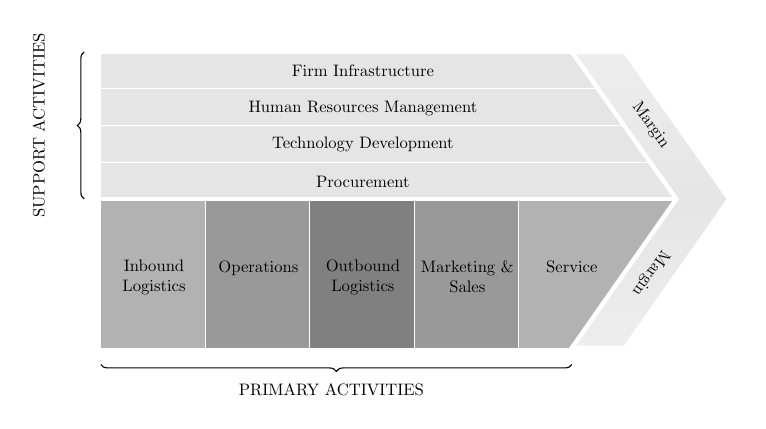
\begin{tikzpicture}[scale=0.8, every node/.style={scale=0.6}]
\matrix (mat) [table]
{
|[fill=colfour]| & |[fill=colfour]| & |[fill=colfour]| & |[fill=colfour]| & |[fill=colfour]| &  \\
|[fill=colfive]| & |[fill=colfive]| & |[fill=colfive]| & |[fill=colfive]| & |[fill=colfive]| &  \\
|[fill=colsix]| & |[fill=colsix]| & |[fill=colsix]| & |[fill=colsix]| & |[fill=colsix]| & |[fill=colsix]| \\
|[fill=colseven]| & |[fill=colseven]| & |[fill=colseven]| & |[fill=colseven]| & |[fill=colseven]| & |[fill=colseven]| \\
|[fill=colone]| & |[fill=coltwo]| & |[fill=colthree]| & |[fill=coltwo]| & |[fill=colone]| & |[fill=colone]|  \\
|[fill=colone]| & |[fill=coltwo]| & |[fill=colthree]| & |[fill=coltwo]| & |[fill=colone]| & |[fill=colone]|  \\
|[fill=colone]| & |[fill=coltwo]| & |[fill=colthree]| & |[fill=coltwo]| & |[fill=colone]| & \\
|[fill=colone]| & |[fill=coltwo]| & |[fill=colthree]| & |[fill=coltwo]| & |[fill=colone]| &  \\
};

% horizontal rules
\foreach \row in {2,3,4}
  \draw[white] (mat-\row-1.north west) -- (mat-\row-6.north east);
\draw[white,ultra thick] (mat-1-1.north west) -- (mat-1-6.north east);
\draw[white,ultra thick] (mat-5-1.north west) -- (mat-5-6.north east);

% vertical rules
\foreach \col in {2,3,4,5}
  \draw[white] (mat-5-\col.north west) -- (mat-8-\col.south west);

% The labels
\node[fill=colfour] at (mat-1-3) {Firm Infrastructure};
\node[fill=colfive] at (mat-2-3) {Human Resources Management};
\node[fill=colsix] at (mat-3-3) {Technology Development};
\node[fill=colseven] at (mat-4-3) {Procurement};
\node at ([yshift=-10pt]mat-6-1) {\parbox[t]{2cm}{\centering Inbound Logistics}};
\node at ([yshift=-10pt]mat-6-2) {\parbox[t]{2cm}{\centering Operations \\\mbox{}}};
\node at ([yshift=-10pt]mat-6-3) {\parbox[t]{2cm}{\centering Outbound Logistics}};
\node at ([yshift=-10pt]mat-6-4) {\parbox[t]{2cm}{\centering Marketing \& Sales}};
\node at ([yshift=-10pt]mat-6-5) {\parbox[t]{2cm}{\centering Service \\\mbox{}}};
\node[rotate = 90] at ([xshift=-52pt]mat-3-1.north) {SUPPORT ACTIVITIES};
\node at ([yshift=-19pt,xshift=-0.5cm]mat-8-3.south) {PRIMARY ACTIVITIES};

\fill[white] (mat-1-5.north east) -- (mat-5-6.north east) -- (mat-1-6.north east) -- cycle;
\fill[white] (mat-8-5.north east) -- (mat-5-6.north east) -- (mat-8-6.north east) -- cycle;

% Draw the arrow tip
\shade[top color=colfour!70,bottom color=colfour!70,middle color=colseven,draw=white,ultra thick] 
  (mat-1-5.north) -- (mat-5-6.north) -- (mat-8-5.south) -- 
  (mat-8-5.south east) -- (mat-5-6.north east) -- (mat-8-5.south east) -- 
  (mat-5-6.north east) -- (mat-1-5.north east) -- cycle;

% "Margin" labels
\begin{scope}[decoration={markings,mark=at position .5 with \node[transform shape] {Margin};}]
\path[postaction={decorate}] 
  ( $ (mat-1-5.north)!0.5!(mat-1-5.north east) $ ) -- ( $ (mat-5-6.north)!0.5!(mat-5-6.north east) $ );
\path[postaction={decorate}] 
  ( $ (mat-5-6.north)!0.5!(mat-5-6.north east) $ ) -- ( $ (mat-8-5.south)!0.5!(mat-8-5.south east) $ );
\end{scope}

% braces
\draw[decorate,decoration={brace,mirror,raise=6pt}]
  (mat-1-1.north west) -- (mat-5-1.north west);
\draw[decorate,decoration={brace,mirror,raise=6pt}]
  (mat-8-1.south west) -- (mat-8-5.south);
\end{tikzpicture}

\caption{Porter's Value Chain}
\end{figure}

\subsection{Data collection}
\subsection{Objectives}
\subsection{Constraints}
\subsection{The Goal Programming model}

\section{Results and Conclusion}

\printbibliography

\end{document}


